\begin{figure}[H]\centering
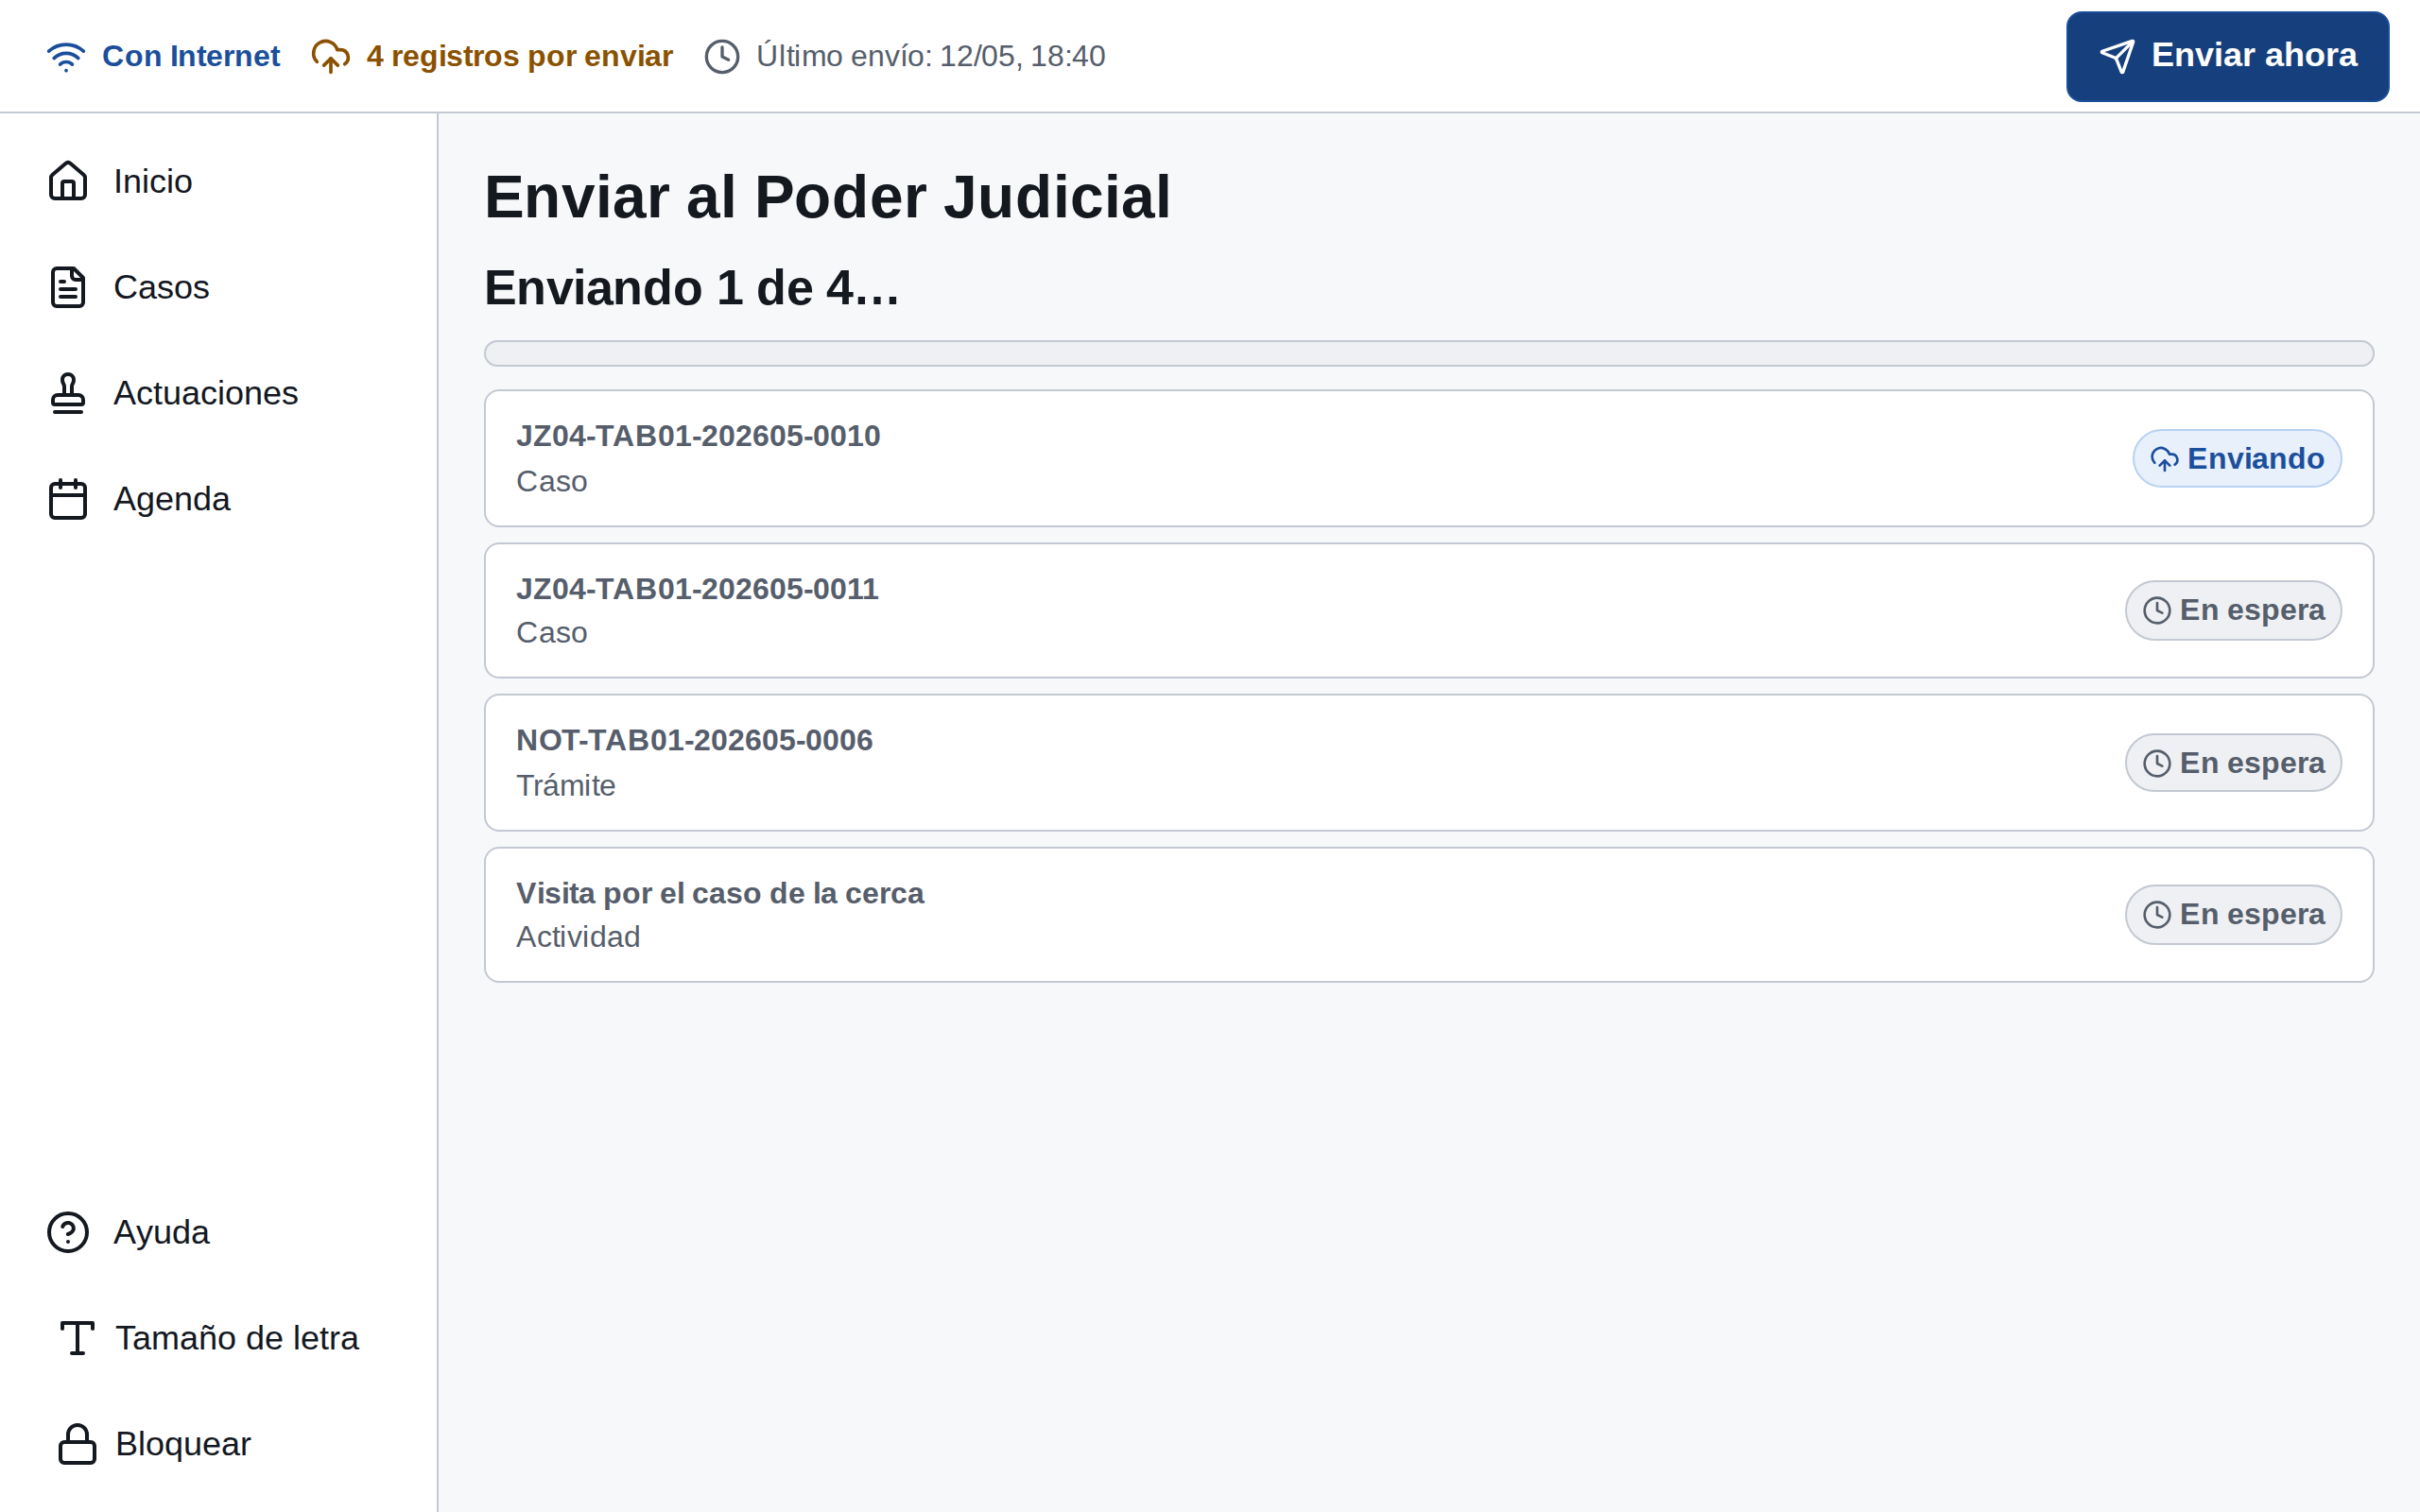
\includegraphics[width=0.82\linewidth]{capturas/P-09a_progreso.png}
\caption{P-09 · Progreso. Progreso con el número de registros y el estado de cada uno}
\end{figure}
\begin{figure}[H]\centering
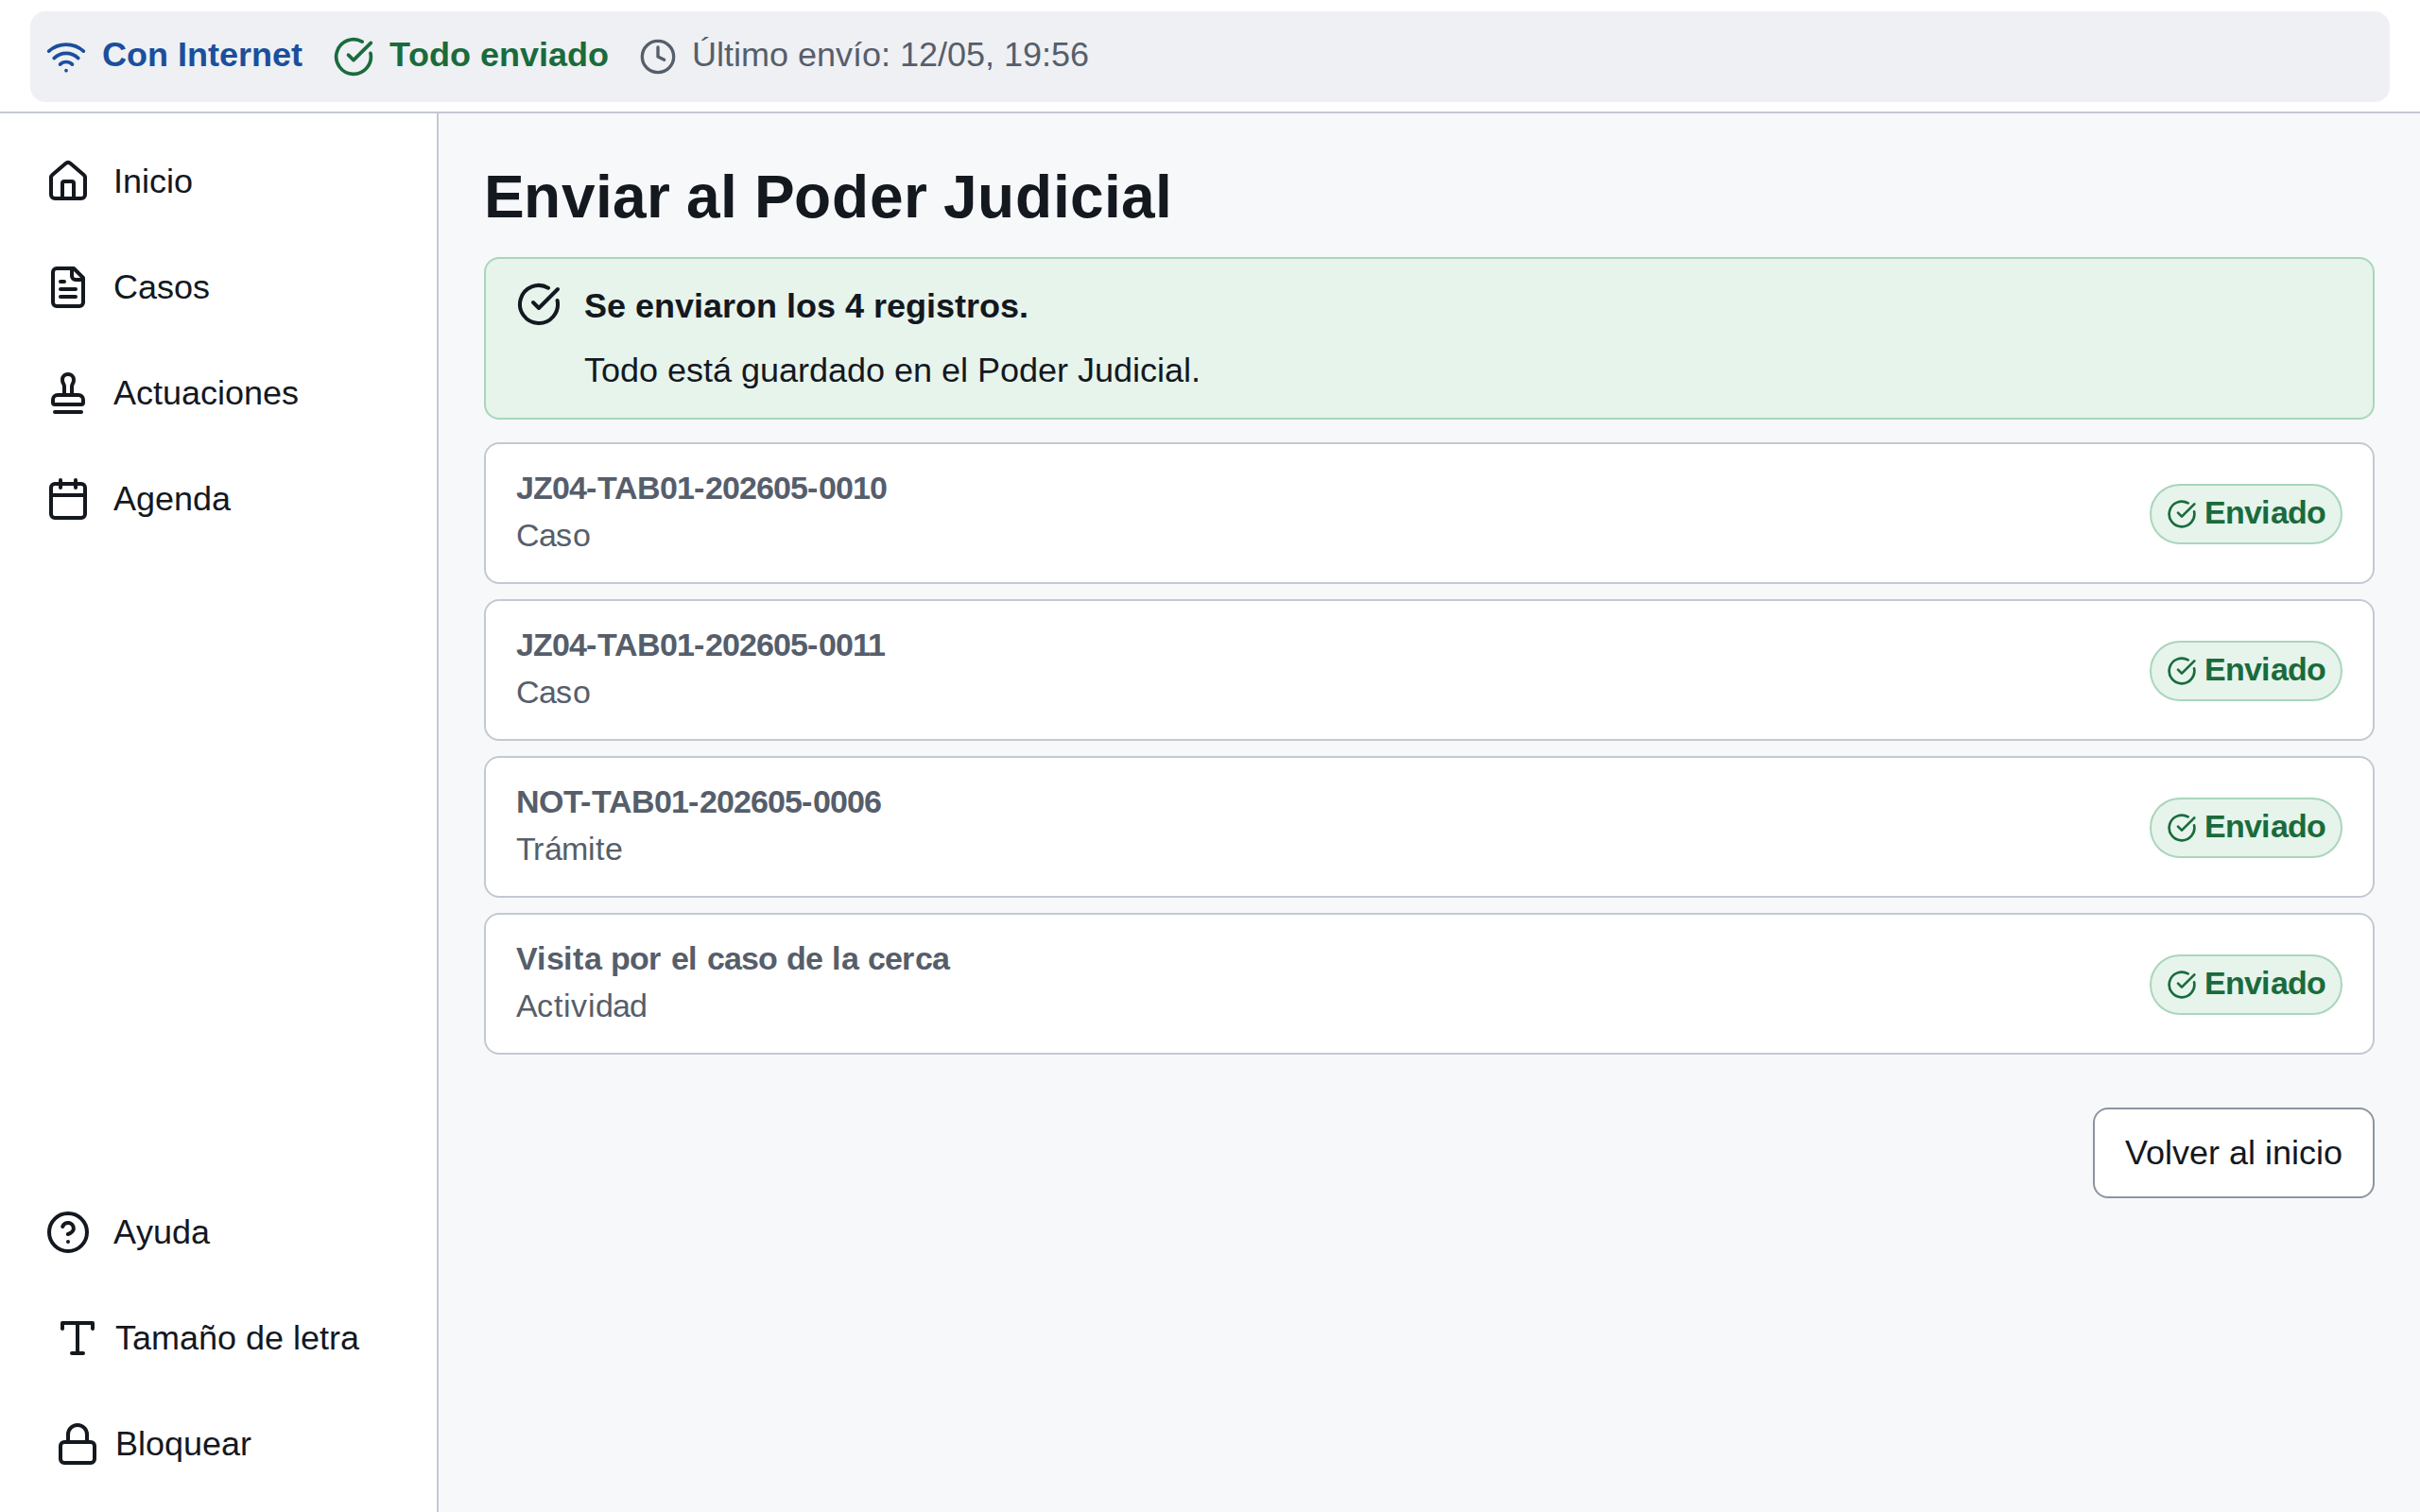
\includegraphics[width=0.82\linewidth]{capturas/P-09b_exito.png}
\caption{P-09 · sync-ok. Se enviaron los 4 registros y la barra pasa a Todo enviado}
\end{figure}
\begin{figure}[H]\centering
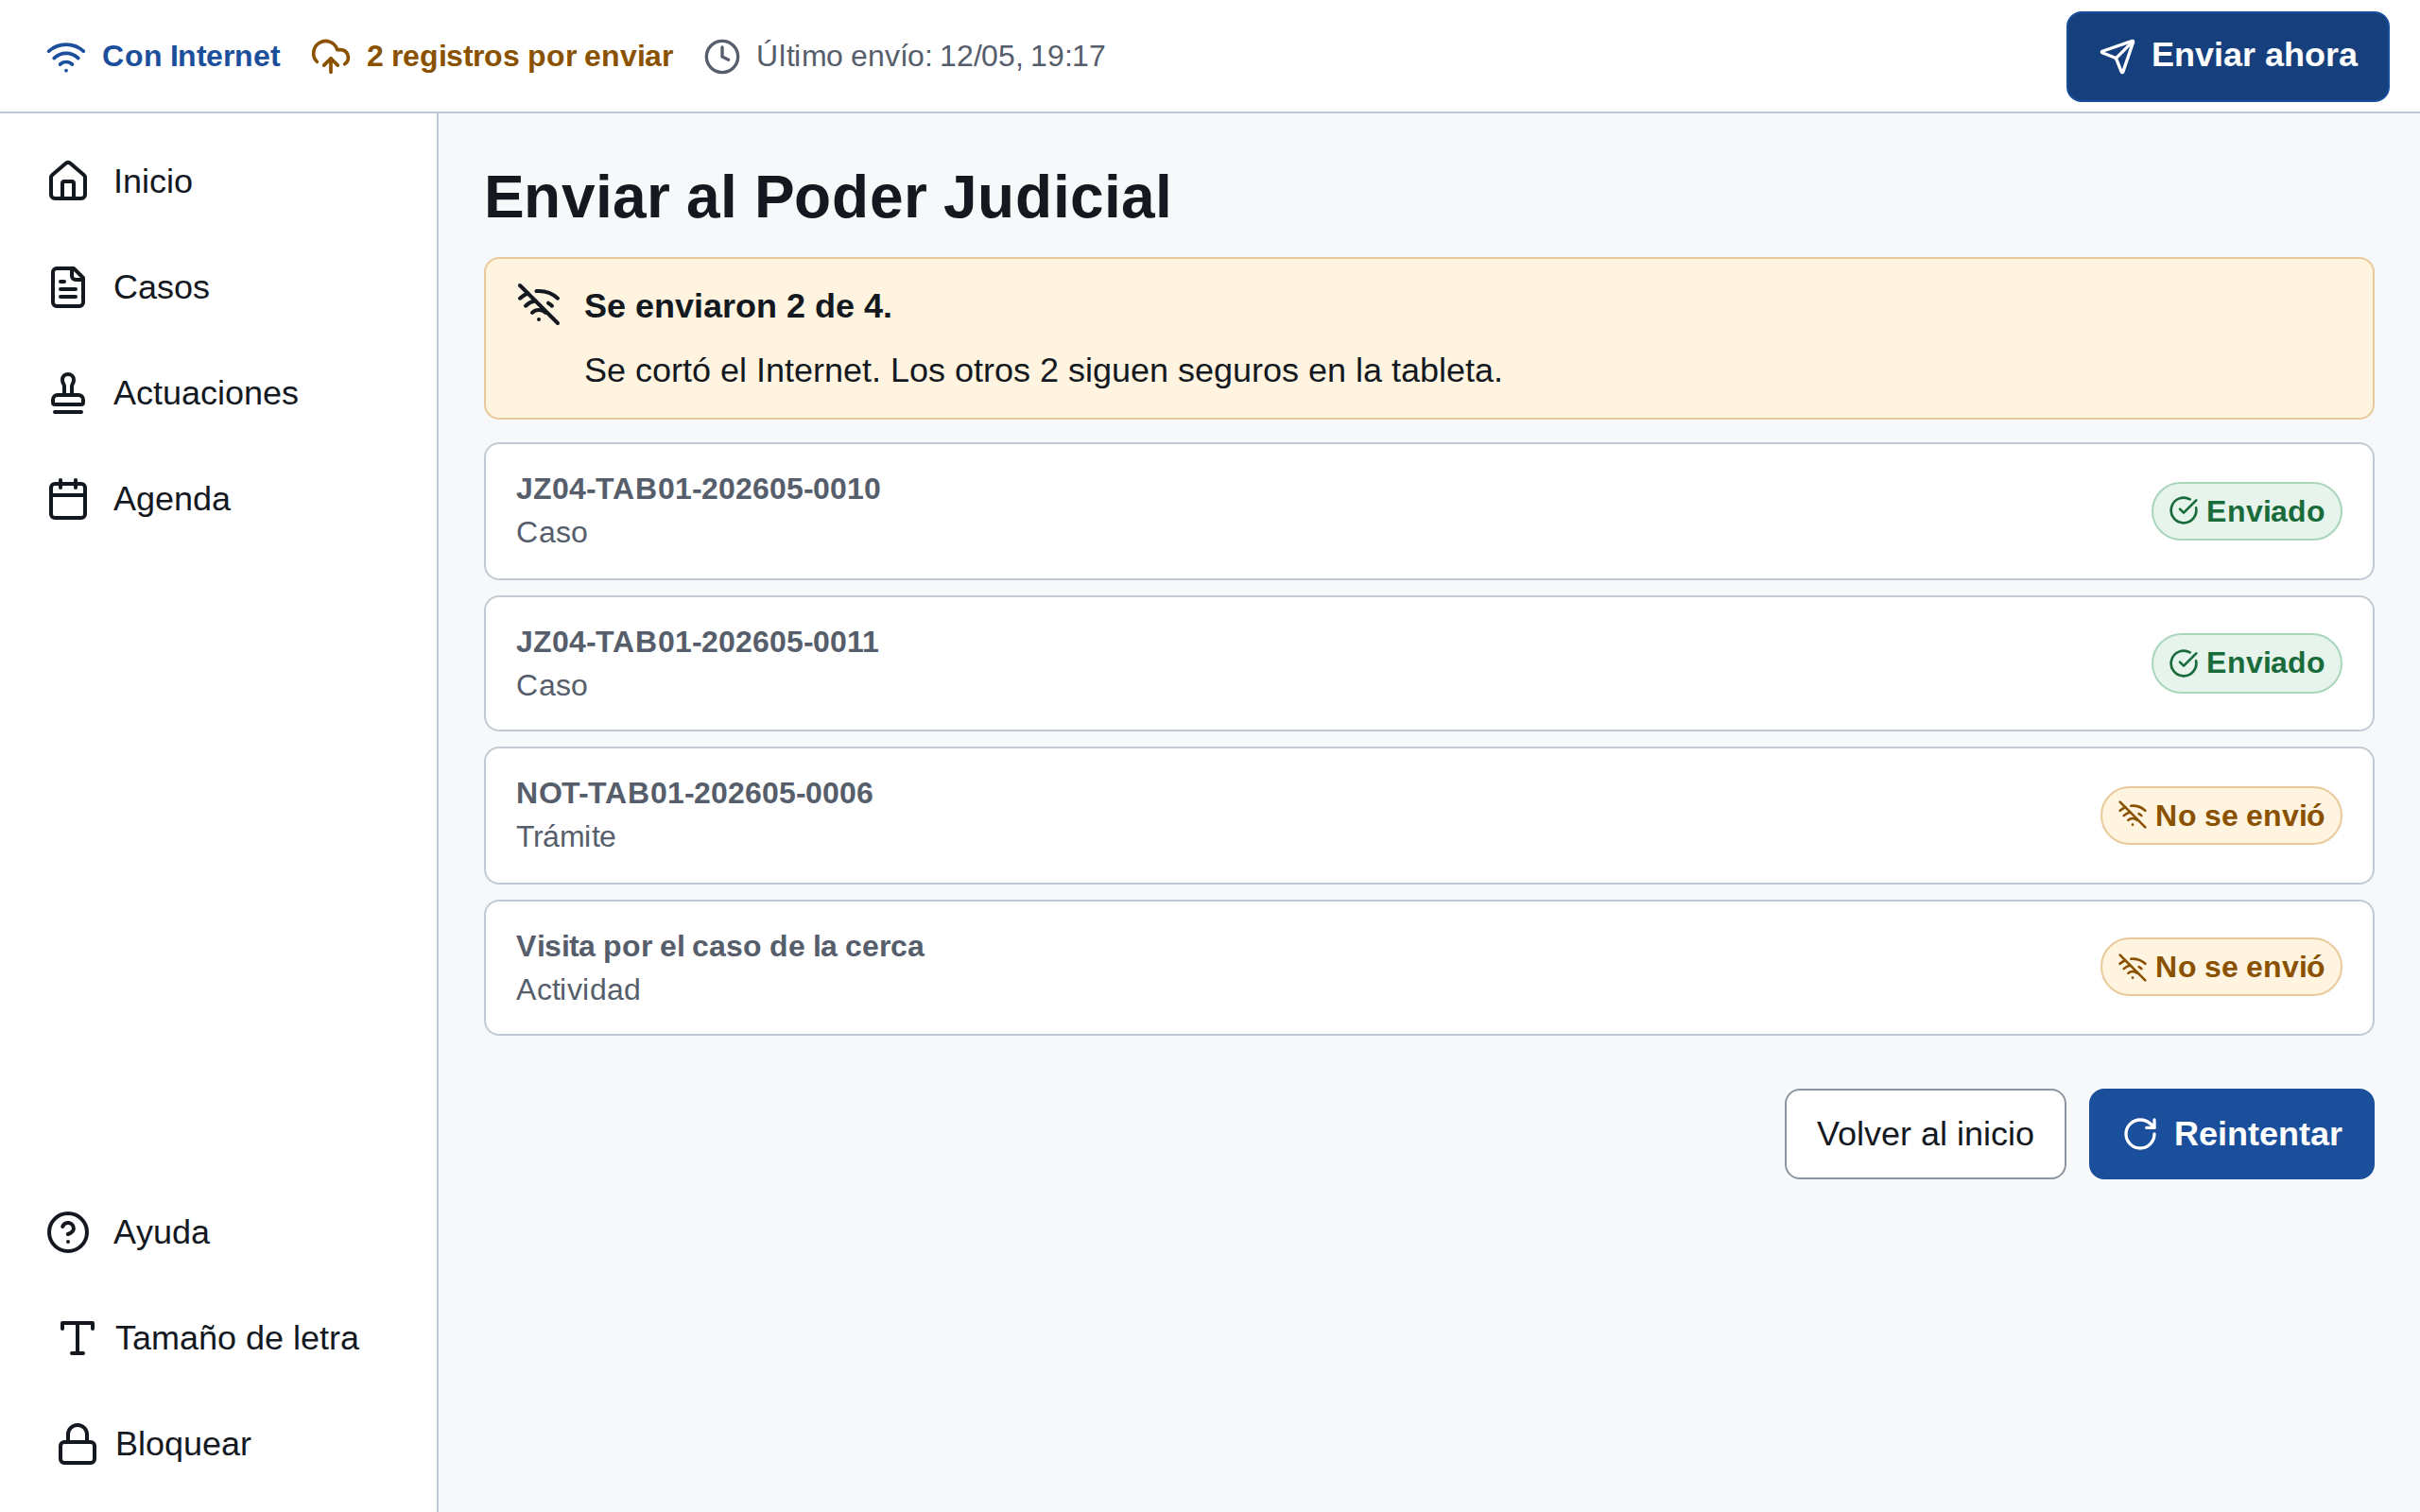
\includegraphics[width=0.82\linewidth]{capturas/P-09c_fallo-parcial.png}
\caption{P-09 · sync-partial. Se cortó el Internet a mitad: dice cuántos llegaron y que el resto sigue seguro}
\end{figure}
\begin{figure}[H]\centering
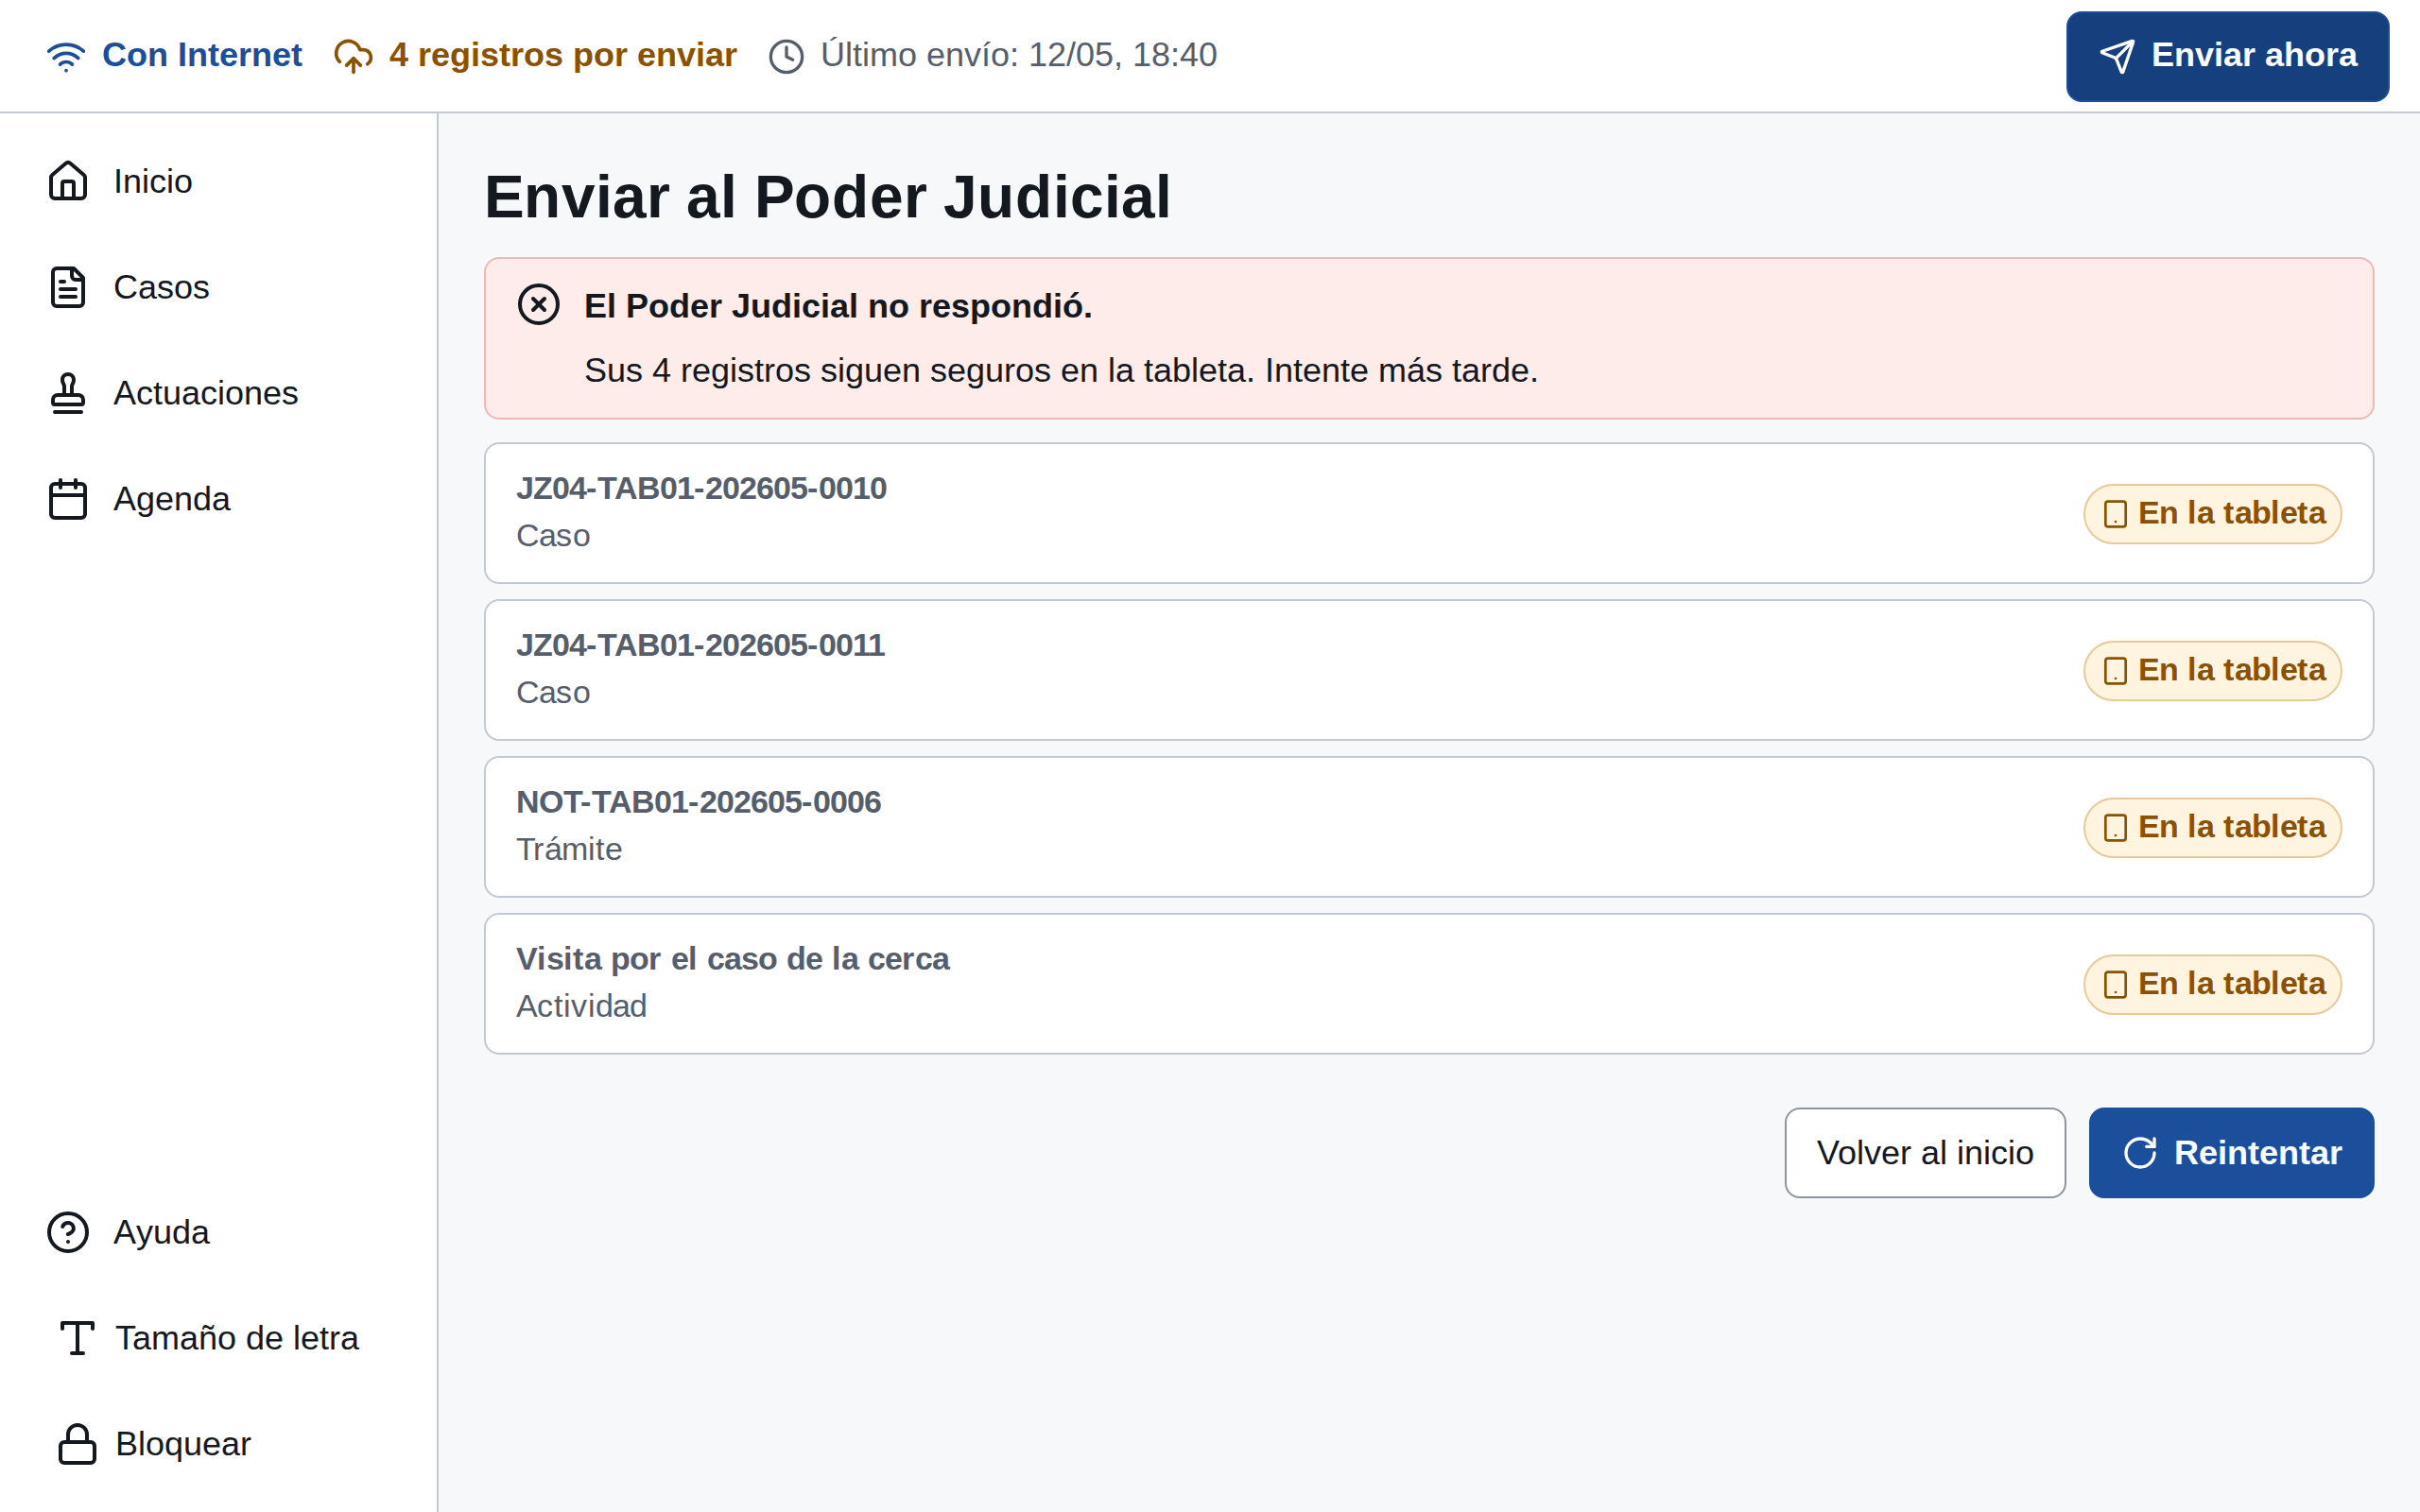
\includegraphics[width=0.82\linewidth]{capturas/P-09d_error-servidor.png}
\caption{P-09 · sync-error. El Poder Judicial no respondió: los registros siguen seguros en la tableta}
\end{figure}
\begin{figure}[H]\centering
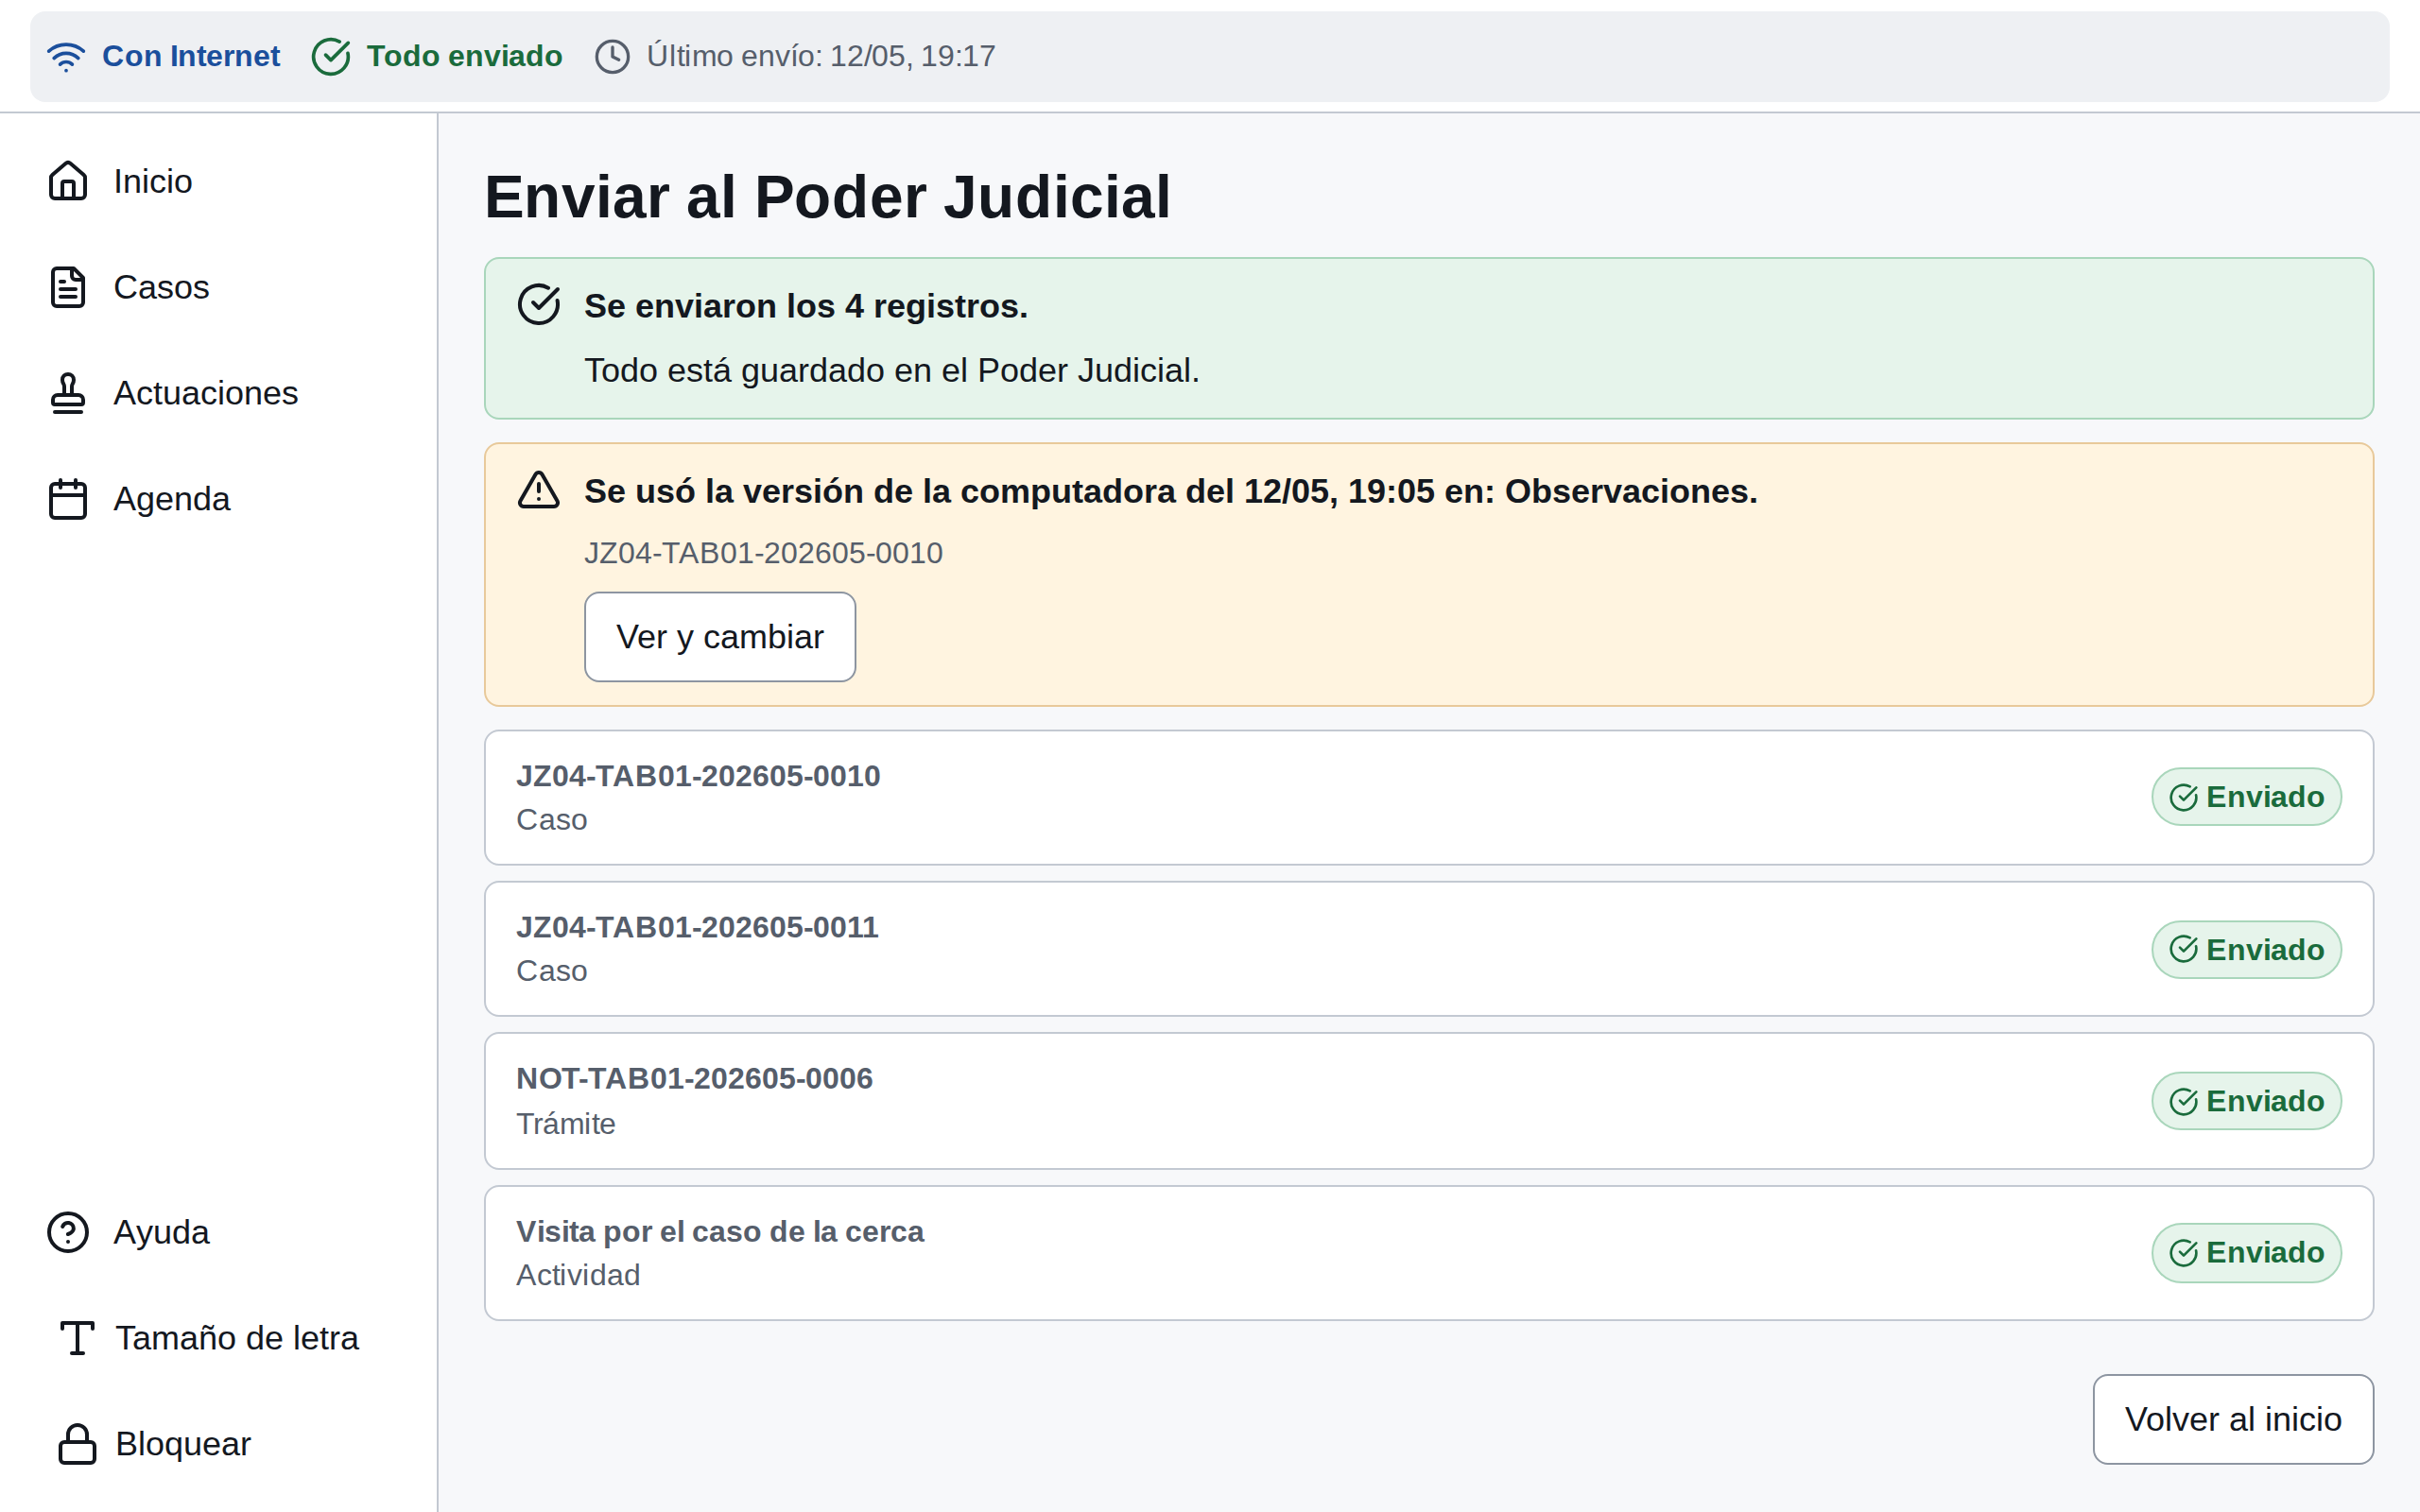
\includegraphics[width=0.82\linewidth]{capturas/P-09e_conflicto.png}
\caption{P-09 · conflict. El conflicto se resuelve solo con el cambio más reciente y se informa qué campo cambió}
\end{figure}
\begin{figure}[H]\centering
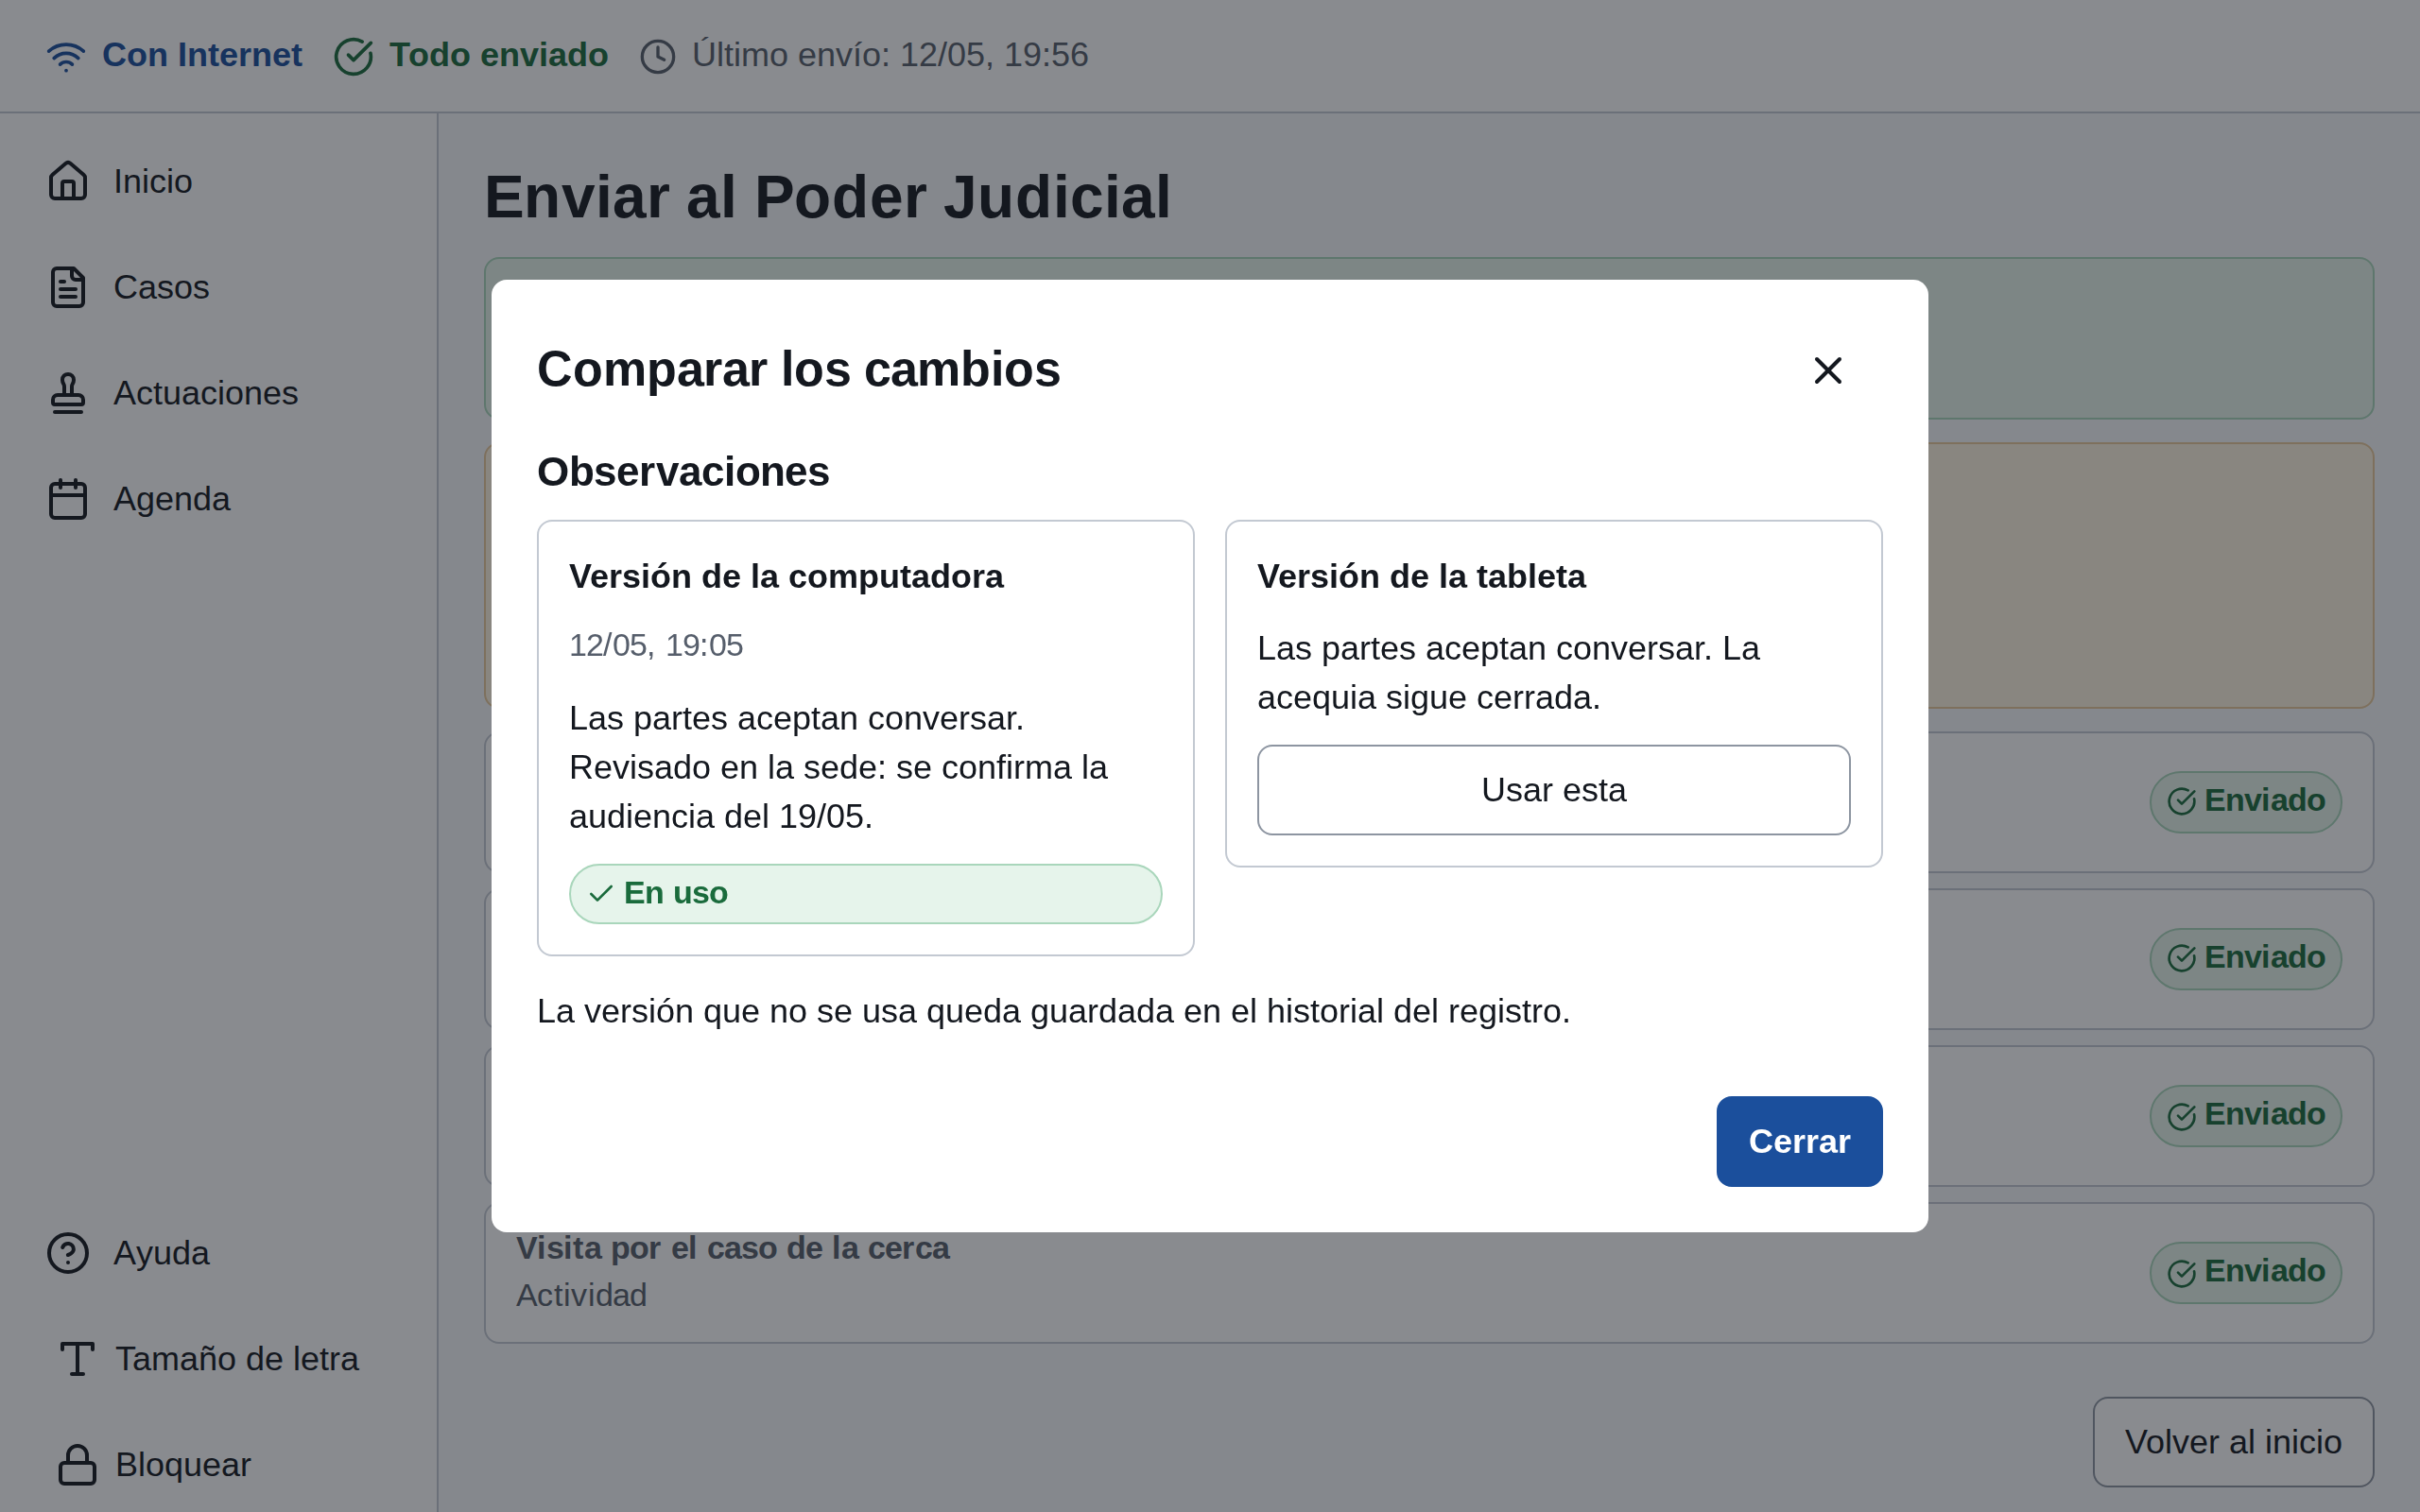
\includegraphics[width=0.82\linewidth]{capturas/P-09f_ver-y-cambiar.png}
\caption{P-09 · Comparación por campo. La comparación campo por campo queda disponible, pero no es obligatoria}
\end{figure}
